\section{The backpropagation algorithm}

\begin{frame}\frametitle{\secname}

The Backpropagation algorithm is a method for computing gradients by using the chain rule efficiently.

\end{frame}


\definecolor{darkgreen}{rgb}{0,0.6,0}
\definecolor{darkcyan}{rgb}{0,0.5,0.5}
\definecolor{darkyellow}{rgb}{0.5,0.5,0}
\definecolor{mangenta}{rgb}{1,0,1}
% -----------------------------------------------------------------------------
\begin{frame} \frametitle{Gradients in neural networks}
	\begin{equation*}
	\textcolor{orange}{	\frac{\partial y(\vec{x}; \vec{w})}{
			\partial \mathrm{w}_{ij}^{v'v}}}
	\end{equation*}

	\begin{center} 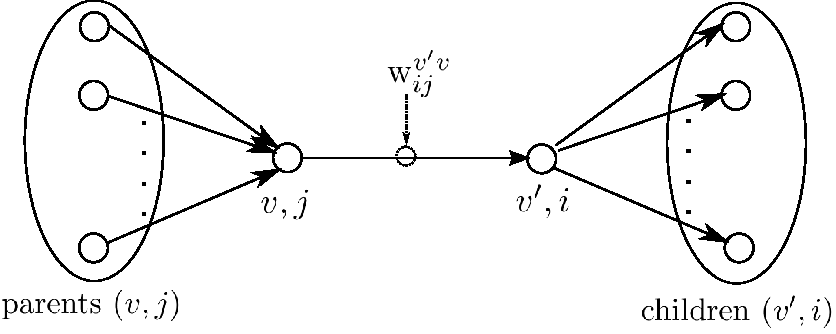
\includegraphics[height=3.5cm]{img/section1_fig20.pdf} \end{center}

		%~ \begin{minipage}{3.5cm}
	\hspace{0.9cm} \tiny Bias node included in the parents.
		%~ \end{minipage}
	\vspace{0.3cm}\\
	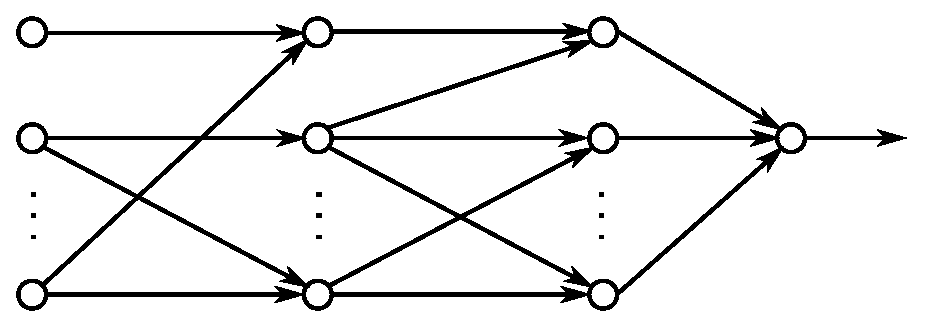
\includegraphics[width=4cm]{img/MLP_horizontal.eps}
	%\hfill{\tiny see blackboard for derivation}
\end{frame}

% -----------------------------------------------------------------------------
\begin{frame} \frametitle{Gradients in neural networks} 

	%\placeimage{9.5}{1}{img/section1_fig20_mini_multicolor.pdf}{width=4.8cm}	
	\vspace{9mm}
	%How do the weights $w_{ij}^{v'v}$ of hidden units $S_i^{v'}$
   	%contribute to the error?
	\begin{block}{Solution: smart application of the chain rule}
		\begin{eqnarray*}
			{\color{darkgreen}h_i^{v'}} 
	   			&=& \kern-2ex\smallsum{(\mu,k) \in P(v',i)}{} \kern-2ex
	   			w_{ik}^{v'\mu}\;  f_k^\mu\big( {\color{teal} h_k^\mu} \big)
	   		\\[4mm]
			\frac{\partial y(\vec{x}; \vec{w})}{\partial \mathrm{w}_{ij}^{v'v}}
				&=& \underbrace{\frac{\partial y(\vec{x}; \vec{w})}
					{{\color{darkgreen}\partial h_i^{v'}}} }_{ 
						\substack{\coloneqq\;{\color{red}\delta_i^{v'}} \\
						\text{``local error''} \\
						\text{at neuron} \\
						(v', i)}
					}
				  \cdot 
				  \underbrace{\frac{{\color{darkgreen}\partial h_i^{v'}}}
				  	{\partial \mathrm{w}_{ij}^{v'v}}}_{
						\substack{=\;f_j^v({\color{teal} h_j^v}) \\
						\text{activity} \\
						\text{of neuron} \\
						(v, j)}}
		\end{eqnarray*}
	\end{block}
\end{frame}

% -----------------------------------------------------------------------------
\begin{frame} \frametitle{Gradients in neural networks}
	%\only<1>{\placeimage{9.5}{1}{img/section1_fig20_mini_multicolor.pdf}{width=4.8cm}}
	%\only<2->{\placeimage{9.5}{1}{img/section1_fig20_mini_back_multicolor.pdf}{width=4.8cm}}
	
	\vspace{11mm}
	\begin{enumerate}
		\item {\textbf forward propagation}: calculate activities 
				$f_i^{v'}({\color{darkgreen}h_i^{v'}})$
				{\small(parents $\rightarrow$ children)}
				$$	
					{
					%\color{darkgreen}
					h_j^0
					} 
						\;:=\; \mathrm{x}_j^{(\alpha)} \,, 
					\quad 
					{\color{darkgreen}h_i^{v'}}
		   			\,= \kern-2ex\smallsum{(\mu,k) \in P(v',i)}{} \kern-2ex
	   			w_{ik}^{v'\mu}\;  f_k^\mu\big( {\color{teal} h_k^\mu} \big) \,,
					\quad
					y(\vec{x}; \vec{w})\,=\, f_1^L({\color{blue}h_1^L})
				$$\\[-2mm]
		\pause
		\item {\textbf backpropagation}: calculate ``local errors'' 
				$\color{red}\delta_i^{v'}$
				{\small(children $\rightarrow$ parents)}
				\vspace{-1mm}
				%~ \begin{eqnarray*} 
				%~ \end{eqnarray*}
				\begin{eqnarray*} 
				{\color{red} \delta_1^L}
				&=& \frac{\partial y(\vec{x}; \vec{w})} {{\color{blue}\partial h_1^{L}}}
					= [f_1^{L}]'({\color{blue} h_1^{L}})
							%\;\;\text{for}\;v'=L
							\\
					{\color{red}\delta_i^{v'}}  
						&=&  \kern-3ex\sum\limits_{(v'', k) \in C(v', i)}
						\underbrace{
							\smallfrac{\partial y(\vec{x}; \vec{w})}
								{{\color{blue}\partial  h_k^{v''}}}
							}_{{\color{red}\delta_k^{v''}}} 
						\;\kern1.5ex\cdot \kern-2.5ex\;
						\underbrace{\smallfrac
								{{\color{blue}\partial h_k^{v''}} }
								{{\color{darkgreen}\partial h_i^{v'}}}
							}_{\mathrm{w}_{ki}^{v''v'} \kern-.5ex\cdot\kern.5ex
								[f_i^{v'}]'({\color{darkgreen}h_i^{v'}}) } %\,,
					\kern-3ex=\;\;\; %\underbrace{
							[f_i^{v'}]'({\color{darkgreen}h_i^{v'}}) 
							\kern-3ex\sum_{(v'', k) \in C(v', i)}\kern-3ex
							{\color{red}\delta_k^{v''}} 
							\mathrm{w}_{ki}^{v'' v'} 
						%}_{{\color{red} \delta_i^L}\;=\;
						%	[f_i^{L}]'({\color{darkgreen} h_i^{L}})
						%	\;\;\text{for}\;v'=L}
				\end{eqnarray*}
		\pause 
		\vspace{-1mm}
		\item {\textbf weight update}: using activities and local errors
			$$
				\mathrm{w}_{ij}^{v'v}
				\quad \leftarrow \quad 
				\mathrm{w}_{ij}^{v'v} - \eta \cdot
				\smallfrac{\partial e\left(y_T, \vec x; \vec w\right)}{\partial\mathrm{w}_{ij}^{v'v}}
				\quad=\quad \mathrm{w}_{ij}^{v'v} - \eta \cdot
				\smallfrac{\partial e\left(y_T, \vec x; \vec w\right)}{\partial y(\vec{x}; \vec{w})} \cdot
				\only<3>{\smallfrac{\partial y}{\partial\mathrm{w}_{ij}^{v'v}}\hspace{8.5mm}}
				\only<4>{{\color{red} \delta_i^{v'}} \kern-.5ex\cdot
			   			f_j^v( {\color{darkgreen}h_j^v} ) }
			$$
	\end{enumerate}
	%{\scriptsize
	%Computational complexity: $O(n)$, $n$: number of weights \& thresholds}
\end{frame}

% -----------------------------------------------------------------------------
\definecolor{forward}{rgb}{0,0.7,0}
\definecolor{backward}{rgb}{0.8,0,0}
\begin{frame} \frametitle{Summary of the backpropagation for gradient descent}
	%\only<1>{
		%\placeimage{10.75}{5.5}{img/MLP_forward.pdf}{width=3.75cm}
		%\placeimage{10.75}{8.7}{img/MLP_backward.pdf}{width=3.75cm}
	%} \only<2> {
		%\begin{minipage}{4}(11.5,5)
			%{\color{blue}
				%\footnotesize
				%\begin{center}
					%computational and 
					%memory complexity \\[2mm]
					%{\color{red}
						%$\mathcal{O}(n)$, %\quad
					%} \\[2mm]
					%$n$: number of weights
					%i.e.~{\em linear} in the 
					%number of weights
				%\end{center}
			%}
		%\end{minipage}
	%}
	
	%\begin{algorithm}[H] 
		%\scriptsize
		\footnotesize
		\DontPrintSemicolon
		initialization of weights and thresholds \\
		\While{stopping criterion not met}{
			$\text{gradient}_{ij}^{v'v} := 0 
					\,, \quad \forall w_{ij}^{v'v}$ \\
			\For{$\alpha \in \{1,\ldots,p\}$}{
				${\color{forward}h_i^0} 
					:= x_i^{(\alpha)} \,, \quad \forall i$ 
				\qquad\qquad // {\color{forward}forward propagation}\\
				\For{$v' \in \{1,\ldots,L\}$}{
					%~ ${\color{forward} h_i^{v'}} 
						%~ := \sum\limits_{\scriptscriptstyle
							%~ (v',i) \in C(v,j)} w_{ij}^{v'v} 
							${\color{forward}h_i^{v'}}
		   			\;\;=\;\; \kern-2ex\smallsum{(\mu,k) \in P(v',i)}{} \kern-2ex
	   			w_{ik}^{v'\mu}\;  \underbrace{f_k^\mu\big( {\color{forward} h_k^\mu} \big) 
								%~ \underbrace{f_j^v({\color{forward} h_j^{v}})
								}_{\kern-2exx_k^{(\alpha)} \;\text{if}\; 
									v'=1\kern-2ex } \,,
							\quad \forall i$
					\vspace{-1.5mm}
				}
				${\color{backward} \delta_1^L} 
					:= [f_1^L]'({\color{forward}h_1^L}) $%\,, \quad \forall i$ 
				\qquad // {\color{backward}backward propagation}\\
				\For{$v' \in \{L-1,\ldots,1\}$} {
					${\color{backward}\delta_i^{v'}} 
						:= [f_{i}^{v'}]'({\color{forward}h_i^{v'}}) 
						\kern-1ex\sum\limits_{(\mu,k) \in C(v',i)}\kern-1ex
						{\color{backward} \delta_k^{\mu}} 
						\, w_{ki}^{\mu v'} \;,
						\quad \forall i$
					\vspace{-2.5mm}
				}
				$\text{gradient}_{ij}^{v'v} := \text{gradient}_{ij}^{v'v}
						+ \frac{\partial e\left(y^{(\alpha)}_T, \vec x^{(\alpha)}; \vec w\right)}{\partial y}
						 \, {\color{backward}\delta_i^{v'}} 
						 \, f_j^v({\color{forward}h_j^v})
						 \,, \quad \forall w_{ij}^{v'v}$
				\hspace{11mm} // sum
			}
			$\text{gradient}_{ij}^{v'v} := \frac{1}{p} \text{gradient}_{ij}^{v'v}$\\
			% $w_{ij}^{v'v} := w_{ij}^{v'v} - \frac{\hat \eta}{p}
			 $w_{ij}^{v'v} := w_{ij}^{v'v} - \eta
					\, \text{gradient}_{ij}^{v'v} 
					\,, \quad \forall w_{ij}^{v'v}	$
			\hspace{15mm} // gradient descent step
					\vspace{-1.5mm}
		}
		%\caption{Backpropagation in feedforward networks}
	%\end{algorithm}
\end{frame}
